%!TEX root = main.tex
\section{Hypothesis Formation and the cycle of visual analysis\label{sec:hypothesis}}
\subsection{Visual Querying in the framework of Data Sensemaking}
In developing \zv, we collaborated with with scientists from astronomy, genetics, and material science in a year-long participatory design process~\cite{Lee2017}. In particular, we study how various features impacts rapid visual querying and analysis, and how a visual query system (VQS) like \zv fit into a scientists’ analysis workflow. Our findings offered design guidelines for improving the usability and adoption of next-generation VQSs. More importantly, in this paper, we focus on applying our findings on visual querying to the context of supporting the full cycle of visual data exploration. We highlight two of the key findings related to this goal below: 

\stitle{Top-down and Bottom-up Querying Modalities}
We employed Pirolli and Card's~\cite{Pirolli} information foraging framework for domain-experts to contextualize our study results. Pirolli and Card's notional model distinguishes between information processing tasks that are \textit{top-down} (from theory to data) and \textit{bottom-up} (from data to theory). In the context of visual querying, users employ top-down approaches by starting with a hypothesis on what patterns to look for and express it through sketching or inputting an equation (Figure~\ref{fig:modalities}b,d). On the other hand, bottom-up approaches originate from the data (or equivalently, the visualization). For example, the user may drag and drop a visualization of interest in the dataset as the input query or upload a visualization from an external dataset (Figure~\ref{fig:modalities}a,c). 
\par Our interactions with the scientists showed that different modalities for inputting a query can be useful for different problem contexts. To our surprise, despite the prevalence of sketch-to-query systems in literature, only two out of our nine users had a practical usage for querying by sketching. Overall, we found that bottom-up querying via drag-and-drop was more intuitive and more commonly used than top-down querying methods, such as sketching or input equations. 
\par One of the main reason why participants did not find sketching useful was that they often do not start their analysis with a pattern in mind. Later, their intuition about what to query is derived from other visualizations that they see in the VQS, in which case it made more sense to query using those visualizations as examples directly. 
\par While -----, formulating top-down queries in a ad-hoc manner can be challenging ---. This ----- why participants did not find top-down querying through inputting equations and sketching ----. \emph{Ad-hoc, sketch-only model for visualization querying is insufficient without }. Despite functional fitting being common in scientific data analysis, Figure \ref{feature_heatmap} shows that querying by equation is also unpopular for similar reasons. In addition, the visualizations for both astronomy and biology exhibit complex processes that could not be written down as an equation analytically. However, even when analytical relationships do exist (in the case of material science), it is challenging to formulate functional forms in an prescriptive, ad-hoc manner. 
\par While the usage of each querying feature may vary from one participant to the next, a key design principle that came from this finding was the need for visual query systems to provide visualization recommendations that can help analysts jumpstart their exploration. Our results indicate that \emph{bottom-up querying approaches are preferred over top-down when the users have no desired patterns in mind}, which is commonly the case for exploratory data analysis. For example, the analyst may examine the top-most similar visualizations that lie in a cluster and finding visualizations that are similar to an object of interest that exhibits a desired pattern. 
%\par For top-down approaches such as query by sketching and input equations, the user starts with an intuition about how their desired patterns should look like based on theory, then queries based on that. 
\par Our \zv work ------- Bottom up and top down querying in VQS facilitates rapid insight discovery. 

\stitle{Construction of multi-step queries}
workflow integration , complex queries,
While our visual interface ---, ----it was unable to capture all the -----. [Give some example queries that didn't work]. Balance between language/querying complexity versus expressiveness. More importantly pointed towards a need for vague querying. Give some examples of vague querying.

\subsection{Supporting cycle of visual data exploration}
Our participatory design findings points towards future ----- in supporting a cycle of ---.  ----advocate ---cycle of visual analysis. 
\begin{itemize}
	\item Essential ingredient in facilitating intelligent vague querying and exploration.
	\item This is a human process (\cite{Heer2012,Pirolli})
	\item Iterative Hypothesis Exploration/Refinement : argue that the following properties is important to sustain this “cycle of visual analysis” 
\end{itemize}

\subsection{Towards 3‘I’s of rapid hypothesis generation support}
Given our observations from the participatory design study, we distill several desiderata for the next generation VQSs. 
Towards 3‘I’s Interactive, Iterative, Informative (Give examples from the ZV-TVCG paper)
\stitle{Interactive flow}:
 (how natural is it to move between analysis steps, facilitate fluid analysis and not get ``stuck'') : interactivity, feedback (latter is quite unexplored), and recommendation, expressivity (how easy is it to express what to do via interactions) and diversity of actions that could be performed.
\stitle{Iterative}: query refinement, dialogue (not a one-shot query)
Joining the flow: Section \ref{sec:vague} focuses on the first two items .
\stitle{Informative}: not just task-based interestingness but more explanation-based (causality, introduce distribution awareness notion in viz-sum), focussed on data understanding, which we will discuss in Section \ref{sec:understanding}

\begin{figure}[h!]
	\label{fig:cycle}
	\centering
	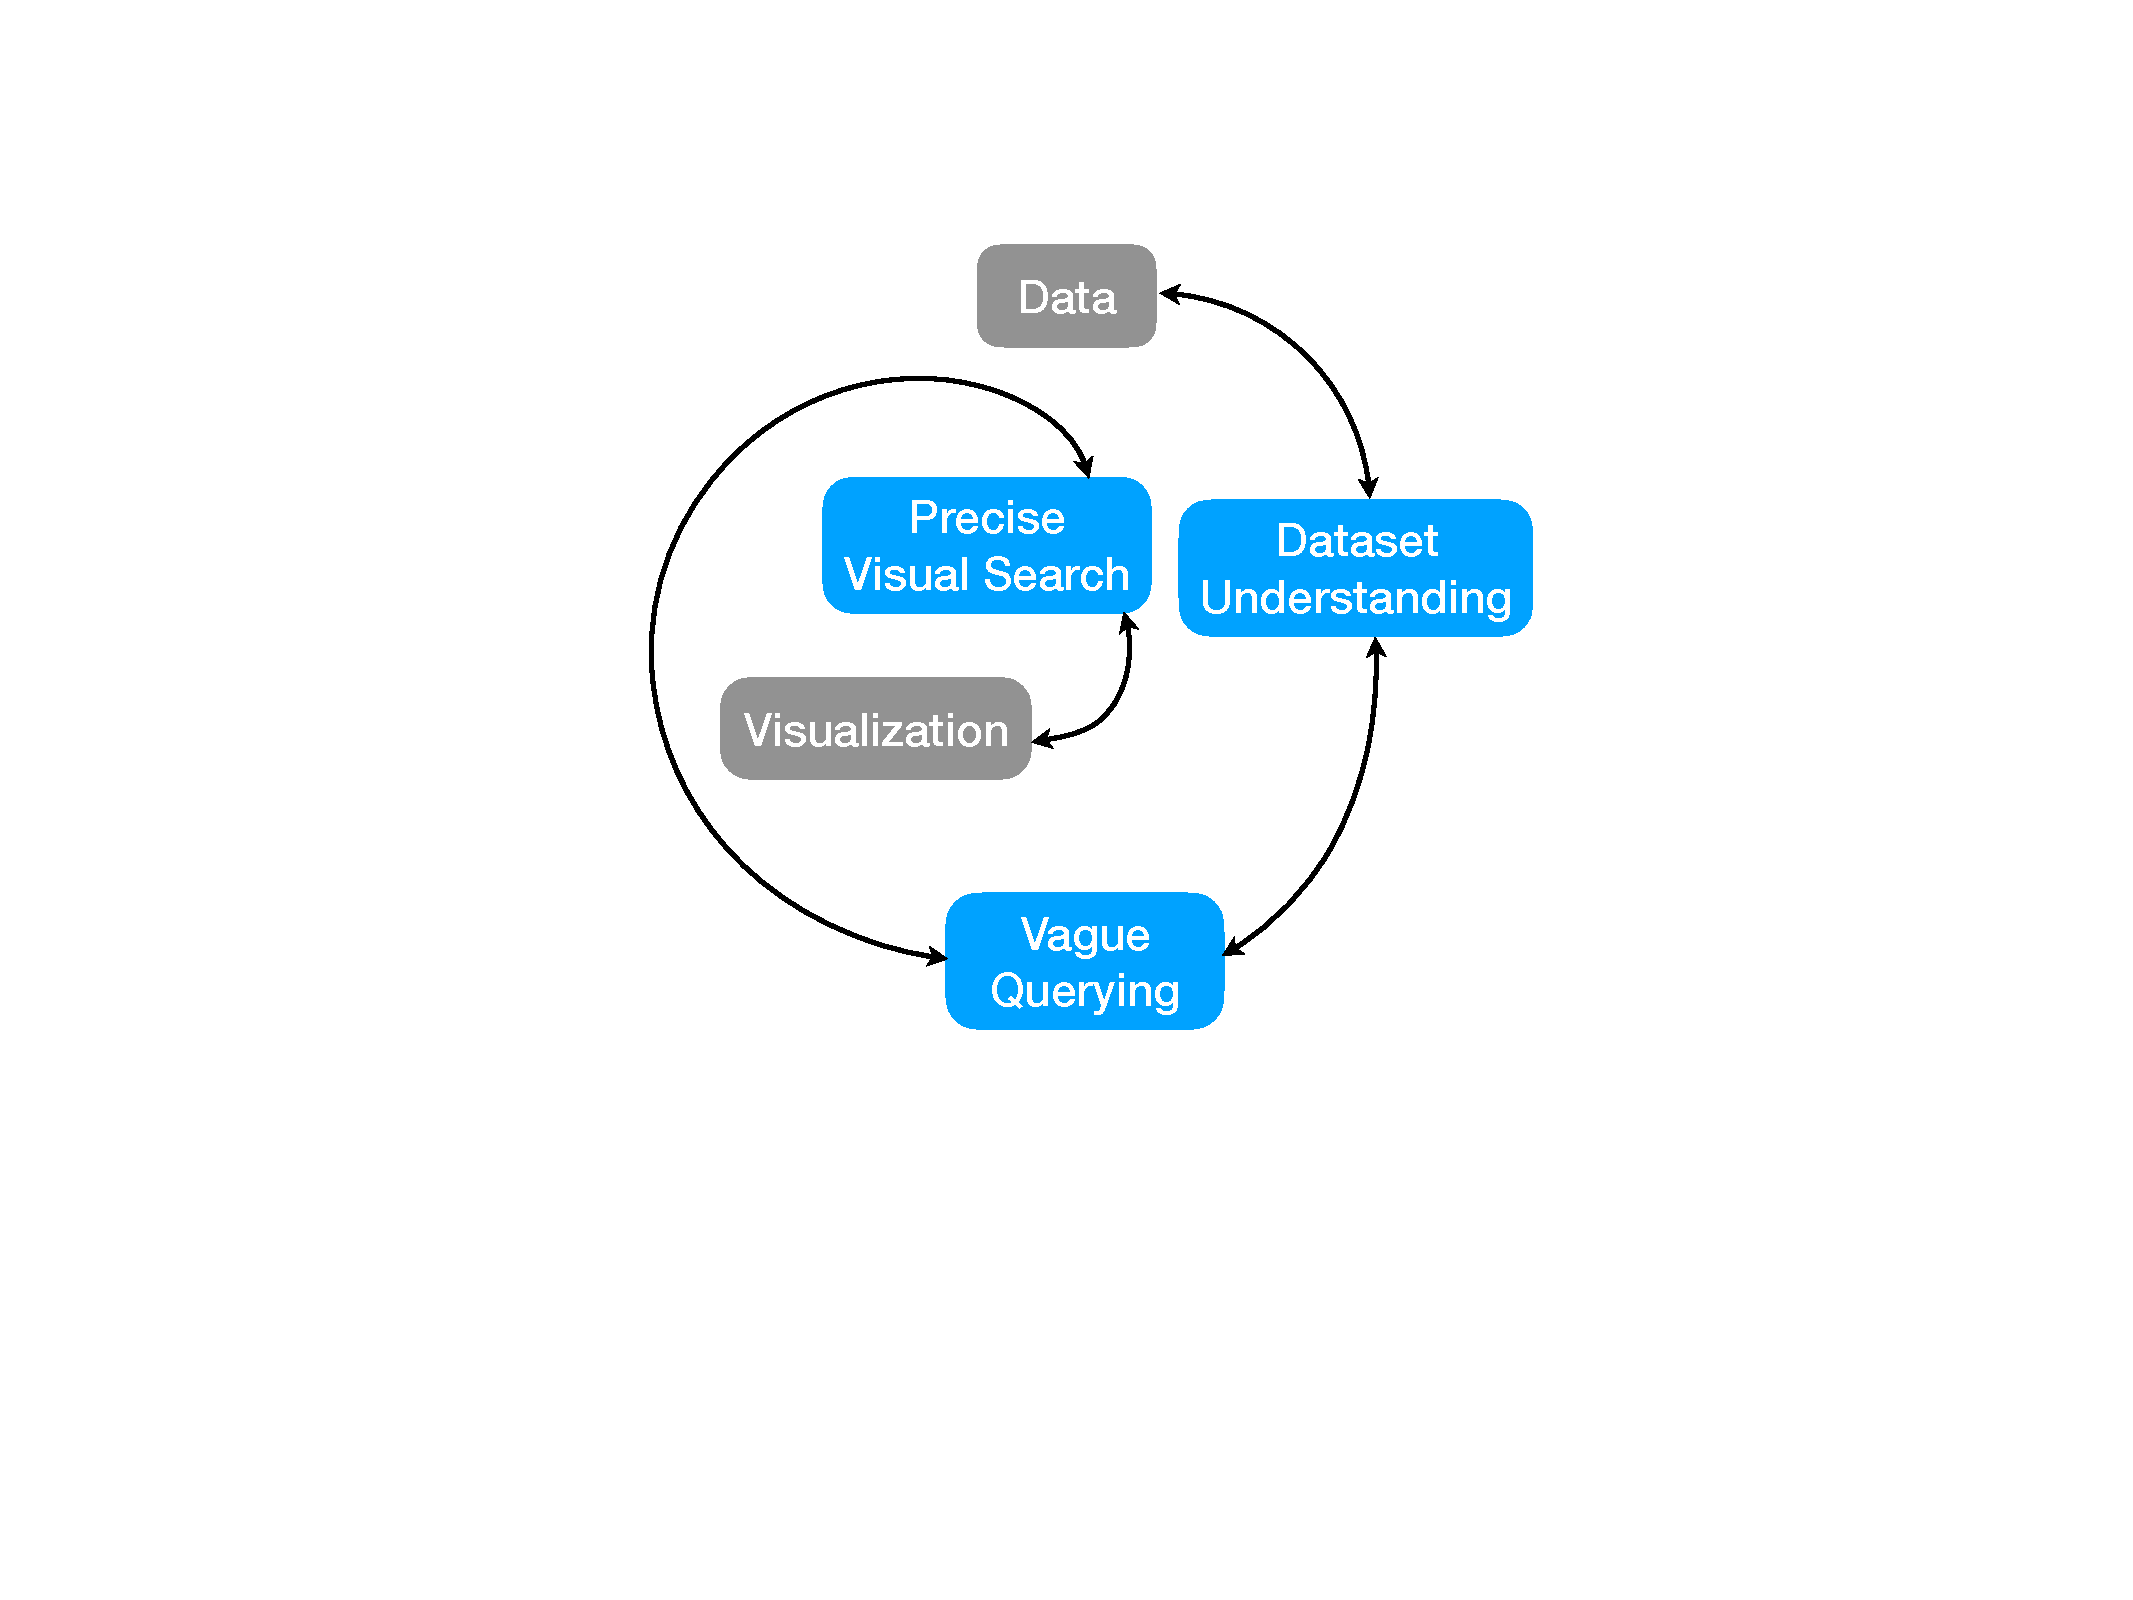
\includegraphics[width=0.5\linewidth]{figures/cycle.pdf}
	\caption{Cycle of visual data exploration.}
\end{figure}

\subsection{Challenges Ahead}
The goal here is to help novice submit precise queries without SQL background, easy to use interface. Our study found that VQS does more than just this, but still not enough.
\begin{itemize}
	\item Precise Search Fail to understand intricacies of user need/intent, need more expressivity/flexibility for querying.
	\item  No perfect training workload, real-world data + task is noisy and complex. 
	\item towards more holistic model for insight discovery
\end{itemize}
